%Journal Alticle Layout by Micah Chambers
%using the IEE bare_jrnl.tex file at 
%% http://www.michaelshell.org/tex/ieeetran/
%% http://www.ctan.org/tex-archive/macros/latex/contrib/IEEEtran/
%% and
%% http://www.ieee.org/

\documentclass[journal]{./IEEEtran}

\usepackage{cite}

\usepackage[pdftex]{graphicx}
\graphicspath{{pdf/}{png/}}

\usepackage[cmex10]{amsmath}
\interdisplaylinepenalty=2500

\usepackage{colortbl}
\usepackage{algorithm}
\usepackage{algorithmic}
\usepackage{array}

\usepackage[caption=false,font=footnotesize]{subfig}
\usepackage{fixltx2e}

\usepackage[colorlinks=true,linkcolor=black,citecolor=black]{hyperref}
\usepackage{url}
\hyphenation{op-tical net-works semi-conduc-tor}

%\begin{comment}
%:Author: Micah Chambers
%:Institution: Virginia Tech University
%\end{comment}

\begin{document}

\title{Full Brain Blood-Oxygen-Level-Dependent Signal Parameter Estimation Using Particle Filters}

%TODO change manuscript recieved/revised
\author{{Micah~Chambers}% <-this % stops a space
\thanks{M. Chambers is with the Department
of Electrical and Computer Engineering, Virginia Tech University, Blacksburg,
VA, 24060 USA e-mail: (micahc@vt.edu}% <-this % stops a space
\thanks{Manuscript received April 19, 2005; revised January 11, 2007.}}

%TODO change journal name
\markboth{Journal of ...}%
{Chambers: Full Brain Blood-Oxygen-Level-Dependent Signal Parameter Estimation Using Particle Filters}
% The only time the second header will appear is for the odd numbered pages
% after the title page when using the twoside option.
% 
% *** Note that you probably will NOT want to include the author's ***
% *** name in the headers of peer review papers.                   ***
% You can use \ifCLASSOPTIONpeerreview for conditional compilation here if
% you desire.

\maketitle

\begin{abstract}
Traditional methods of analyzing FMRI images use a linear combination of
just a few static regressors. This work demonstrates an alternative
approach using a physiologically inspired nonlinear model. By using a 
particle filter to optimize the model parameters, the computation time
is kept below a minute per voxel without requiring a linearization 
of the noise in the state
variables. The activation results show regions similar to those found in 
SPM; however, there are some notable regions not detected by 
SPM. Though the parameters selected by the particle filter based approach
are more than sufficient to predict the BOLD response,
more model constraints are needed to uniquely identify a single set
of parameters. This ill-posed nature explains the large discrepancies
found in other research that attempted to characterize the model parameters.
For this reason the final distribution of parameters is more medically relevant
than a single estimate. Because the output of the particle filter is 
a full posterior probability, the reliance on the mean to estimate 
parameters is unnecessary. This work presents
not just a viable alternative to the traditional method of detecting
activation, but an extensible technique of estimating the joint probability
distribution function of the BOLD parameters.
\end{abstract}

% Note that keywords are not normally used for peerreview papers.
\begin{IEEEkeywords}
BOLD Response, FMRI, Nonlinear Systems, Particle Filter, Bayesian Statistics, System Identification
\end{IEEEkeywords}

% For peer review papers, you can put extra information on the cover
% page as needed:
% \ifCLASSOPTIONpeerreview
% \begin{center} \bfseries EDICS Category: 3-BBND \end{center}
% \fi
%
% For peerreview papers, this IEEEtran command inserts a page break and
% creates the second title. It will be ignored for other modes.
\IEEEpeerreviewmaketitle

\section{Introduction}
\label{sec:Introduction}
% The very first letter is a 2 line initial drop letter followed
% by the rest of the first word in caps.
% 
% form to use if the first word consists of a single letter:
% \IEEEPARstart{A}{demo} file is ....
% 
% form to use if you need the single drop letter followed by
% normal text (unknown if ever used by IEEE):
% \IEEEPARstart{A}{}demo file is ....
% 
% Some journals put the first two words in caps:
% \IEEEPARstart{T}{his demo} file is ....
% 
% Here we have the typical use of a "T" for an initial drop letter
% and "HIS" in caps to complete the first word.
\IEEEPARstart{T}{raditional} methods of analyzing 
Functional Magnetic Resonance Imaging (FMRI)
time series perform regression using a linear 
combination of static explanatory variables. 
However, the static nature of the General Linear Model (GLM)
limits its potential use. It is well known that different 
Hemodynamic Response Functions are necessary 
for different regions of the brain to prevent excessive false
negatives \cite{Handwerker2004}. Additionally quite a few studies
have reported spatially varying nonlinearities \cite{Wager2005,Birn2001}.
Besides not allowing HRF differences between patients, there is no
reasonable way to incorporate other forms of physiological
data. Combined FMRI CBF or CBV imaging methods are improving,
as seen in Chen et al. \cite{Chen2009}. These techniques could shed light on
neural activation by providing extra measurements, yet a 
physiologically reasonable model is necessary to incorporate this extra data.
Activation detection methods also don't have the ability 
to identify pathologies based on state variables or parameters. For
example, decreased compliance of blood vessels could indicate, or 
even cause, a neurological condition that 
is not easily seen in other imaging modalities. 

It is well known that the changes in deoxy-hemoglobin content is the
primary driver of short term changes in MR signal for FMRI imaging
techniques \cite{Buxton1998, WEISSKOFF1994, Ogawa, Obata2004}. For
this reason, the nonlinear state equations that change Deoxy-Hb (DHb) 
content have been heavily studied, and are well-characterized. Attempts
at learning the parameters of the BOLD model have also been actively
studied but significantly less successful. The most wide-spread method
of calculating the parameters, from two papers by Friston et al., 
are part of the SPM toolkit; though this algorithm is rarely used 
as well \cite{Friston2000, Friston2002b}. 
This method depends on a quadratic convolution (two term Volterra Kernel)
based estimation of the BOLD output to obtain partials with respect 
to parameters. Problematically, quality of the Volterra estimate
is not well known, so it is difficult to quantify error. This method 
also doesn't account for noise in the parameters or the state variables.

These shortcomings have led to several other separate attempts. In particular 
Riera et al. linearized the noise and thus performed regression between
the model and steps of the BOLD output \cite{Riera2003}. This aproach
had the benefit of a Jacobian,  but at the same time removes all DC 
signal. For this reason, the type of activation limits the
algorithms' ability to learn the model.
In Vakorin et al., a combination of Genetic Algorithms and Simulated 
Annealing were used to estimate not only the parameters, but the 
true stimuli driving the BOLD signal \cite{Vakorin2007}. 
This addresses the inherent uncertainty of exactly where and when 
stimuli actually get applied. Unfortunately this algorithm was extremely
slow; taking hours or days per single time course.
In Johnston et al. alternating estimates of $P(X_t | \Theta, Y_t)$ and 
$P(\Theta | Y_t)$ were calculated, to maximize $P(X_t, \Theta | Y_t)$. 
$P(X_t | \Theta, Y_t)$ was calculated using a particle filter 
\cite{Johnston2008}. This however was quite slow, and the results
were inconsistent with other similar works. 
Murray used a particle filter, similar to \cite{Johnston2008}, but
held the model parameters constant; thus all error in the output
was treated as the result of noise in the underlying parameters 
\cite{Murray2008}. Murray's results showed that differences in
BOLD output cannot be well explained by error in the state variables.
Hu et al. used an unscented kalman filter (UKF) to estimate parameters,
and filtered parameter sets inconsistent with the output  \cite{Hu2009}.
 Furthermore, Birn et al. and Yacoub et al. showed that many
of the characteristics of the BOLD output depend on the region 
of interest \cite{Birn2001, Yacoub2006}. For this reason, a single
Hemodynamic Response Function is not likely to accurately estimate
activation across the full brain. 

With the exception of Hu et al., the works described thus far all
worked to estimate a single set of parameters that could
explain the output \cite{Hu2009}. Yet Deneux et al showed that the very similar
outputs can be achieved with very different parameters \cite{Deneux2006}.
This explains the inconsistencies in parameters across the different
studies. Thus, estimating parameters using a least squares
framework is not likely to be fruitful; and though the posterior
distributions will vary spatially, that difference will not be
discernible from a single parameter estimate. The problem with 
using an Unscented Kalman Filter to approximate the distributions
is that with a nonlinear, dissipative system, significant non-Gaussian
effects will be present. In tests, significant non-Gaussian effects 
began to appear within a second of state integration. With FMRI
repetition times being well above 1 second, a Gaussian approximation
will result in significant error. The particle filter, which can be
thought of an extension of UKF, uses non-parametric distributions
rather than a Gaussian. For this reason the particle filter, described
in \autoref{sec:ParticleFilters}, is used in this work.

\section{Methods}
\label{sec:Methods}
\subsection{Bold Model}
\label{sec:BoldModel}
In the past fifteen years, a steady stream of studies have built
on the original Blood Oxygen Level Dependent (BOLD) signal 
derivation first described by Ogawa et al. \cite{Ogawa}.
The seminal work by Buxton et al. attempted to explain the
time evolution of the BOLD signal using a windkessel model to
describe the local changes in Deoxygenated Hemoglobin content \cite{Buxton1998}.
Incremental improvements were made to this model until Friston et al.
brought all the changes together into a single complete 
set of equations \cite{Friston2000}. And while there have been numerous adaptations in the model, 
many of them summarized by Deneux et al., even the basic versions
have less bias error than the empirically driven 
\emph{Canonical Hemodynamic Model} \cite{Deneux2006,Handwerker2004}.
On the other hand BOLD signal models have numbers
of parameters ranging from seven \cite{Riera2003} to 50 \cite{Behzadi2005} 
for a signal as short as 100 samples long. This number of parameters presents
a significant risk of being under-determined and having high computation cost. 
In this work, only the simplest physiologically inspired model will be
used (with 7 parameters), and steps will be taken to make the most of computation
time.

It is well known that the two types of hemoglobin act as a contrast agents in 
EPI imaging \cite{Buxton1998, WEISSKOFF1994, Ogawa}, however the connection
between Deoxyhemoglobin/Oxygenated Hemoglobin and neural activity is non-trivial. 
Intuitively, increased metabolism will increase Deoxyhemoglobin, 
however blood vessels are quick to compensate by increasing local 
blood flow. Increased inflow, accomplished by loosening 
capillary beds, precedes increased outflow, driving increased 
blood storage.  Since the local MR signal depends on the ratio of 
Deoxyhemoglobin to Oxygenated Hemoglobin, increased blood volume 
affects this ratio if metabolism doesn't exactly match the increased 
inflow of oxygenated blood.  This was the impetus
for the ground breaking balloon model \cite{Buxton1998} and windkessel
model \cite{Mandeville1999}. These works derive, from first principals,
the changes in deoxyhemoglobin ratio and volume of capillaries given an 
inflow waveform.  These were the first two attempts to quantitatively 
account for the shape of the BOLD signal as a consequence of the lag 
between the cerebral blood volume (CBV) and the inward cerebral blood 
flow (CBF). 

Although Buxton et al. demonstrated that a well chosen flow waveform could 
explain most features of the BOLD signal, it stopped short of proposing a
realistic waveform for the CBF and CMRO2 \cite{Buxton1998}. Friston et al. 
gave a reasonable and simple expression for CBF input based on a flow 
inducing signal and in the same work proposed a simple method
of estimating metabolic rate: as a linear function of the inward 
blood flow \cite{Friston2000}. By combining these equations with 
the balloon model from Buxton et al., it is possible to predict 
the BOLD signal directly from a stimulus time course:
\begin{eqnarray}
\dot{s} &=& \epsilon u(t) - \frac{s}{\tau_s} - \frac{f - 1}{\tau_f} \\
\dot{f} &=& s\\
\dot{v} &=& \frac{1}{\tau_0}(f - v^\alpha)\\
\dot{q} &=& \frac{1}{\tau_0}(\frac{f(1-(1-E_0)^f)}{E_0} - \frac{q}{v^{1-1/\alpha}})
\label{eq:bold}
\end{eqnarray}
where $s$ is a flow inducing signal, $f$ is the input blood flow (CBF),
$v$ is normalized cerebral blood volume (CBV), and $q$ is the normalized
local deoxyhemoglobin. The parameters controlling blood flow are 
$\epsilon$, which is a neuronal efficiency term, $u(t)$ which is 
the stimulus, and $\tau_f$, $\tau_s$ which are time constants. 
The parameters for the evolution of blood volume are $E_0$ which 
the resting metabolic rate and $\alpha$ which is Grubb's parameter 
controlling the balloon model.  $\tau_0$ is a single time constant 
controlling the speed of $v$ and $q$.

This completed balloon model was assembled and analyzed
by Riera et al. \cite{Riera2003}. Obata refined the readout equation 
of the BOLD signal based on the deoxyhemoglobin content ($q$) and local 
blood volume ($v$), resulting in the final BOLD equation \cite{Obata2004}.
\begin{eqnarray}
y   &=& V_0((k_1 + k_2)(1-q) - (k_2 + k_3)(1-v))\\
k_1 &=& 4.3 \times \nu_0 \times E_0 \times TE = 2.8 \nonumber \\
K_2 &=& \epsilon_0 \times r_0 \times E_0 \times TE = .57 \nonumber \\
k_3 &=& \epsilon_0 - 1 = .43 \nonumber
\label{eq:boldout}
\end{eqnarray}
Where $\nu_0 = 40.3 s^{-1}$  is the frequency offset in Hz for fully
de-oxygenated blood (at 1.5T), $r_0 = 25 s^{-1}$  is the slope relating
change in relaxation rate with change in blood oxygenation, and
$\epsilon_0 = 1.43$ is the ratio of signal MR from intravascular to 
extravascular regions at rest. Although, these constants change with 
experiment ($TE$, $\nu_0$, $r_0$), patient, and brain 
region ($E_0$, $r_0$), often the estimated values by Obata et al. are 
taken as the constants $a_1 = k_1 + k_2 = 3.4$, and $a_2 = k_2+k_3 = 1$ in 
studies using 1.5 Tesla scanners \cite{Obata2004}.
Additional compartments and parameters have been added since 
Riera et al., however Deneux et al. showed that only the viscoelastic
effects of Buxton et al. were necessary to model the primary 
elements of the BOLD response \cite{Riera2003, Deneux2006, Buxton2004}.
Despite this, only the basic balloon model of Buxton et al. is
used in this work, although future works may benefit from constraining
the parameters as described by Deneux et al. \cite{Buxton2004, Deneux2006}.

\subsection{Particle Filter}
\label{sec:ParticleFilters}
Particle filters, a type of Sequential Monte Carlo (SMC) method,
are a powerful method for estimating the posterior probability distribution
 of parameters given a time series of measurements. Unlike Markov 
Chain Monte Carlo (MCMC) estimation, particle filters are designed for 
time-varying random variables. Unlike the UFK, sample points are kept
and continuously propagated forward, rather than being used to calculate
the first two moments. Thus, the posterior distribution is
stored as an empircal distribution made up of sample points.
Particle filters are preferred when the model is nonlinear, 
and non-Gaussian. This section based primarily on 
Arulampalam et al. and Thrun et al. \cite{Arulampalam2002a, Thrun2005}.

The idea of the particle filter is to build an empirical distribution
out of a large number of parameter sets, called particles. Each
particle contains all the parameters and states needed to propagate
the model forward.  The particle filter begins with a wide distribution 
(called the Prior Distribution)
of possible particles and then, as measurements come in, weights 
particles based on the quality of their output estimates. Thus parameter sets 
that tend to give good estimations of the measurements get weighted higher
than parameter sets that give poor estimates. Although the reliance on
a prior distribution could be problematic, when the system being modeled
has physical meaning, establishing reasonable ranges for parameters may be 
quite easy. Optimizing the prior distribution can be more difficult,
unless the system has been extensively studied.

\subsubsection{Assumptions}
Suppose a set or stream of measurements at discrete times are given, 
$\{Y_k, k = 1, 2, 3, ... K\}$, where $K$ may be infinite. 
Because $k$ is a discrete time, let $t_k$ define the continuous
time of $k$.
Suppose also that there is a hidden set of state variables,
$X(t)$ that drives the value of $Y(t)$. Throughout this section
with $X_k = X(t_k)$. The goal of the particle filter is to estimate the 
distribution of the
true parameters $\Theta$ that dictates the movement of $X(t)$.
The model also permits random motion in $X(t)$, so the 
particle filter also estimates the distribution of $X(t)$.
The only difference between the members of parameter vector
$\Theta$ and those of $X(t)$ is that the memebers of
$\Theta$ have no known update equation. Members of both vectors
are permitted to have some noise, although this
may not be explicitly stated in the model. The generic, continuous, nonlinear
system definition is shown in \autoref{eq:GenericNonlinear}.

\begin{eqnarray}
\dot{X}(t) = f(t, X(t), u(t), \theta, \nu_x) \nonumber \\
Y(t) = g(t, X(t), u(t), \theta, \nu_y)
\label{eq:GenericNonlinear}
\end{eqnarray}

$X(t)$ is vector of state variables, $\Theta$ is a vector of system
constants, $u(t)$ is an input, $Y(t)$ the observation, and
$\nu_x$ and $\nu_y$ are random variates. Although any of these
variables could be a vector, for the sake of simplicity only
$\Theta$ and $X(t)$ will be considered as such. 

I will also make a few  simplifying assumptions for this work. 
First, the systems are assumed to be 
time invariant. This 
assumption is based on the idea that if you paused the system for $\Delta t$
seconds, when unfrozen the system would continue as if nothing happened. 
Few biological systems are predictable enough for them to be summarized
by a time varying function, least of all the brain. While heart beats are certainly
periodic and have an effect on the BOLD signal, the period varies too much
for the system to be considered varying with time. 
Next, its assumes that input cannot directly
influence the output, which in the case of the BOLD signal is a good assumption.
Finally, because the only difference between the members of $X(t)$ and 
$\Theta$ is an update function, from now on $X$ will encapsulate
$\Theta$. The assumptions allow for a simplified version of the
state space equations:

\begin{eqnarray}
\dot{X}_k &=& f(X_{k-1}, u_k, \nu_x)
\label{eq:stateass}\\
Y_k &= &g(X_k, \nu_y)
\label{eq:measass}
\end{eqnarray}

\subsubsection{Prior Distribution}
The goal of the particle filter is to evolve an empirical distribution 
$P(x_k | u_{0:k}, Y_{0:k})$,
that asymptotically approaches the true probability distribution $P(X_k | u_{0:k})$.
Note that capital $X$ will be used as the actual realizations of 
the state variable, whereas $x$ will denote estimates of $X$.
Additionally, the notation $a:b$ indicates the set $[a,b]$,
as in $u_{a:b}$, which would indicate all the inputs from time $a$ to time $b$.
Considering the noise present in $X$,
 $P(X_k | u_{0:k})$ is not a single true value but probability distribution. 

To begin with, the particle filter must be given a prior distribution, from
which the initial $N_p$ particles are drawn. A particle contains a weight
as well as an estimate of $X_k$, which as previously mentioned, contains every
variable needed to run the model. Then the prior is generated from a 
given distribution, $\alpha(X)$, by:

\begin{equation}
\{(x^i_0,w^i) : x^i_0 \sim \alpha(X), w^i = 
            \frac{1}{N_p} : i \in \{1, 2, ... , N_p\} \}
\end{equation}

Where $N_p$ is the number of particles or points used to 
describe the prior using a Mixture PDF.  Note that any 
exponents will be explicitly labeled as such, to avoid 
confusion with the particle numbering scheme. 

Therefore, as $N_p \rightarrow \infty$:
\begin{equation}
\alpha(X) \approx P(x_0) = \sum_{i=0}^{N_p} w^i\delta(X - x^i_0 ) dx
\end{equation}
Where $\delta(x-x_0)$ is 1 if and only if $x = x_0$
(the Kronecker delta function).
$\alpha(X)$, the prior distribution, \emph{must} cover the 
true posterior distribution in order for the particle filter
to converge to the true posterior distribution.

\subsubsection{Basic Particle Filter}
For all the following areas, the probabilities implicitly depend on $u_{0:k}$, 
so they are left off for simplicity.
Whenever a measurement becomes available it permits refinement of the
posterior density.  Incorporating new data is called sequential 
importance sampling. The weight of a particle in an empirical distribution
is defined as
\begin{equation}
w^i_k \propto \frac{P(x^i_{0:k} | y_{0:k})}{q(x^i_{0:k} | y_{0:k})}
\label{eq:weightfunc}
\end{equation}
where $q$ is called an \emph{importance density}. The importance density
is the density of the particles, thus by dividing by this value, the weight
should not depend on the location of the estimation points, but rather
only on $P(x^i_{0:k} | y_{0:k})$, the probability of that particle
being correct given all the measurements up to time $k$. 
Note that if there is a far off peak in
the posterior that $q$ does not have support points in, there will 
be quantization errors, and that part of the density cannot be modeled. 
This is why $q$ must fully cover $P(x^i_{0:k} | y_{0:k})$.

To update the weight of a particular particle at time $k$, it is necessary to 
calculate both $q(x^i_{0:k} | y_{0:k})$ and $P(x^i_{0:k} | y_{0:k})$, 
in \autoref{eq:Support} and \autoref{eq:UpdateBayes} respectively.

Note that $q(x^i_{0:k} | y_{0:k})$ may be simplified by assuming that 
$y_k$ doesn't contain any additional information about $x_{k-1}$. 
\begin{equation}
q(x^i_{0:k} | y_{0:k}) = q(x^i_{0:k} | y_{0:k-1})
\label{eq:QAssump}
\end{equation}
The choice of the importance density, $q(x_k | x_{k-1}, y_{0:k})$ is 
a design decision; however it is common to use the state model: 
\begin{equation}
q(x_k | x_{k-1}, y_{0:k}) =  P(x_k | x_{k-1})
\label{eq:ImportanceDensity}
\end{equation}
This choice for importance density is helpful because 
$P(x_k | x_{k-1})$ is freely available: its simply the set 
of particles propagated forward in time using the state 
equations. Additionally it makes
updating weights simple, as seen later (\autoref{eq:weightevolve}).
$q(x^i_{0:k} | y_{0:k})$ may then be simplified:
\begin{equation}
q(x_{0:k} | y_{0:k}) = P(x_k | x_{k-1})q(x_{0:k-1} | y_{0:k-1})  
\label{eq:Support}
\end{equation}

Calculating $P(x_{0:k} | y_{0:k})$ 
uses the assumption that the distribution of $y_k$ is 
fully constrained by $x_k$, and that $x_k$ is similarly fully 
constrained by $x_{k-1}$, I make the good assumptions that:
\begin{eqnarray}
P(y_k | x_{0:k}, y_{0:k-1}) &=& P(y_k | x_k) \nonumber \\
P(x_k | x_{0:k}, y_{0:k-1}) &=& P(x_k | x_{k-1})
\label{eq:MarkovProperty}
\end{eqnarray}
These are restatements of the state equations assumed by \autoref{eq:stateass}
and \autoref{eq:measass}.
Additionally, for the particle filter $y_k$ and $y_{0:k-1}$ are 
constant across all particles, thus $P(y_k| y_{0:k-1})$ can
be dropped when the equality is changed to a proportion. 
Using these properties and Bayes' Theorem, $P(x^i_{0:k} | y_{0:k})$ 
may be broken up as follows:
\begin{equation}
P(x_{0:k} | y_{0:k}) \propto P(y_k| x_k) P(x_k | x_{k-1}) P(x_{0:k-1} | y_{0:k-1}) 
 \label{eq:UpdateBayes}
\end{equation}

Plugging \autoref{eq:ImportanceDensity} and the result of \autoref{eq:UpdateBayes}
into \autoref{eq:weightfunc} leads to:
\begin{eqnarray}
w^i_k & \propto & \frac{P(y_k| x^i_k)  P(x^i_{0:k-1} | y_{0:k-1})}
                         {q(x^i_{0:k-1} | y_{0:k-1})} \nonumber \\
& \propto & w^i_{k-1}P(y_k| x^i_k) 
\label{eq:weightevolve}
\end{eqnarray}

Thus, by making the following simple assumptions, evolving a posterior
density  requires no knowledge of noise distribution.
\begin{enumerate}
\item $f(t, x(t), u(t)) = f(x(t), u(t))$ and $g(t, x(t), u(t)) = g(x(t))$ 
\item The prior distribution PDF, $q(x_i(0))$, covers $P(x_i(0))$
\item Markov Property: $P(x_k | x_{0:k-1}) = Pr(x_k | x_{k-1})$
\item $q(x_{0:k-1} | y_{0:k}) = q(x_{0:k-1} | y_{0:k-1})$
\end{enumerate}

From the definition of $w_i$, the algorithm to calculate
an approximation of $P(X(t_k) | Y_{0:k})$ or $P(X(t_k + \delta t) | Y_{0:k})$
is simple (see Algorithm \autoref{alg:BasicParticleFilter}). 

\subsubsection{Sequential Importance Resampling}
\label{sec:ParticleFilterResampling}
As a consequence of the wide prior distribution 
(required for a proper discretization of a continuous
distribution), a significant proportion of particles quickly
develop insignificant weights. 
Ideally the computation time spent on tails would be proportional to 
the actual size of the tails.  The case where a large number of the 
weights have become extremely small
is called particle degeneracy. In  Lui et al. 
an ideal measurement of degeneracy based on the particles' true 
weight is given \cite{Liu1998b}. An approximation of 
the effective number of particles is also given: 
\begin{equation}
N_{eff} \approx \frac{\sum_{i=0}^{N_p} w_i}{\sum_{i=0}^{N_p} w_i^2}
\label{eq:neff}
\end{equation}
To alleviate particle degeneracy, a technique known as resampling 
may be applied. The idea of resampling is to 
draw from the approximate posterior, thus generating 
a replica of the posterior probability with 
a matching support. Each particle in the new distribution,
$\hat{x}_j$, is drawn from the old distribution 
(see Algorithm \autoref{alg:Resampling}):
\begin{equation}
\hat{x}_j \sim \left(\sum_{i=0}^{N_p} w^i_k\delta(x - x^i_k)\right)
\end{equation}

For infinite particles this new distribution will match the old.
Unfortunately, in practice since the support is
limited to the original particles, the number of \emph{unique} 
particles can only decrease.
This effect, called particle impoverishment, can result in 
excessive quantization errors in the final distribution. 
To prevent particle impoverishment, instead of sampling from the
discrete distribution, a smoothing kernel is applied.
Because the distribution is continuous, particle impoverishment
is prevented. This regularization process is defined as:
\begin{equation}
x_i = x_i + h\sigma \epsilon
\end{equation}
Where $h$ is an optional bandwidth, $\sigma$ is the standard 
deviation such that $\sigma \sigma^T = cov(x)$
and $\epsilon$ is drawn from the chosen kernel. In this case
a Gaussian kernel was used, and the bandwidth was set to 1
(see \autoref{alg:RegResampling}). All the 
pseudocode may be found in \autoref{sec:algorithms},
including the complete regularized particle filter used
(Algorithm \autoref{alg:RegularizedParticleFilter}).
\begin{table}[t]
\centering
\begin{tabular}{|c || c | c | c |}
\hline
Parameter & Distribution & $\mu$ & $\sigma$ \\
\hline
$\tau_0$ & Gamma & .98 & .25 \\
$\alpha$ & Gamma & .33 & .045\\
$E_0$    & Gamma & .34 & .03  \\
$V_0$    & Gamma & .04 & .03 \\
$\tau_s$ & Gamma & 1.54  & .25\\
$\tau_f$ & Gamma & 2.46  & .25\\
$\epsilon$ & Gamma & .7  & .6 \\
\hline
\end{tabular}
\caption{Prior distributions used in the particle filter.}
\label{tab:Prior}
\end{table}
\autoref{eq:weightevolve} still depends on knowing
$P(y_k| x^i_k)$. Ideally this would exactly match the
measurement error distribution of the system; however,
even if this distribution is incorrect, the solution will
still converge. For this work it was assumed that
\begin{equation}
P(y_k | x^i_k) = g(X_k, \nu_y) = g(X_k) + \nu_y\text{, }\nu_y \sim N(0, 0.005^2)
\end{equation}
A standard deviation of $0.005$ performed well in the general case, primarily
because the BOLD signal tends to be in the range of $0.01-0.05$, (1\%-5\%).
Additionally, 1400 Euler integration points were used per second, 
the system was assumed to start at rest. The system was initialized
with 16,000 particles, but during the first resampling, the number
of particles was dropped to 1,000. To prevent over-smoothing, resampling
was only performed when $\N_{eff}$ (\autoref{eq:neff}) dropped below
$50$ for two consecutive measurements. 

\subsection{Preprocessing}
The BOLD response has been
extensively studied and despite minor discrepancies, the cause of the BOLD
signal is well known. However, FMRI has an extremely low SNR. 
A particularly difficult form of noise present 
in FMRI is a low frequency
drift, often characterized as a Wiener process \cite{Riera2004}.
Though not present in all regions, as many as ten to fifteen percent
of voxels can be affected, thus it is prevalent 
enough to cause significant inference problems \cite{Tanabe2002, Smith2007}. 
Though the cause is still not
clear it is clear that this drift signal is not solely
due to a physiological effects, given its presence in cadavers and phantoms
\cite{Smith1999}. The problem mandates the use of a high pass 
filter \cite{Smith2007}.  In a comparison of high pass filters,
Tanabe et al.  showed that generally subtracting off
a spline improved the SNR the most \cite{Tanabe2002}.

To prevent transients at the beginning of the FMRI run, the first 9
measurements (18.9 seconds) were dropped. Each of the remaining 
images were registered to the new first image, to account for
movement. 
One knot was used for every 20 time points (at a TR of 2.1), with the first
knot and last knot taking half as many points as the rest of the knots.
The median level of each group of measurements was calculated, and the
knot placed at the average time of the group. After subtracting this spline
from the timeseries, the resulting timeseries was divided by the original
sample mean. To compensate for the BOLD signal not generally being zero-mean,
the Median-Absolute-Deviation was added to the final signal (\autoref{eq:mad}). 
\begin{equation}
y_{\text{gain}, 0:K} = 1.4826\underset{i=0:K}{\text{median}}(y_i - 
        \text{median}(y_{0:K}))
\label{eq:mad}
\end{equation}

For SPM, the first 9 measurements were again dropped, and the images
co-registered across time. The co-registered data was spatially smoothed,
and then filtered with an adaptive cut off (which is built into the
SPM analysis). For the SPM analysis, the Canonical HRF was used
and model time derivatives were included (but not in the contrast
vector). All other settings used in SPM8 were left at the default
for analyzing FMRI data.

\subsection{Simulation}
\label{sec:MethodsSim}
\begin{table}[t]
\centering
\begin{tabular}{|c |c | c | c | c | c | c | c |}
\hline
Region & $\tau_0$ & $\alpha$ & $E_0$    & $V_0$    & $\tau_s$ & $\tau_f$ & $\epsilon$  \\
\hline
1 & 1.454& 0.321& 0.369& 0.036& 0.994& 2.774& 1.348\\
2 &1.151&  0.353& 0.380& 0.026& 1.98&  2.333& 1.645 \\
3 &1.951&  0.317& 0.348& 0.027& 1.657& 3.719& 0.757 \\
4 &1.203 & 0.310& 0.326& 0.036& 2.168& 2.272& 0.086\\
\hline
\end{tabular}
\caption{Actual parameters for each regions in the POSSUM simulated slice.
Regions shown in \autoref{fig:simslice_mask}.}
\label{tab:simsliceparams}
\end{table}

Single voxel simulations were performed by propagating the BOLD
model forward through time with 2000 integration points per
second, then adding I.I.D. Gaussian noise and a Wiener process
with I.I.D. steps. For all single voxel simulations,
the signal was generated using the following parameters:
$\{\tau_0 = 1.45, \alpha = 0.3, E_0 = 0.47, V_0 = 0.044, 
\tau_s = 1.94, \tau_f = 1.99, \epsilon = 1.8\}$,
with measurement noise ($\sigma_y$) of $0.001$ and drift standard deviation
($\sigma_x$) of $0.0005$. Two separate tests are discussed in the
results. A single voxel test was performed with for 2400 seconds with random
stimuli (Poisson distributed, $\lambda = 1$ event per second) lasting 
$0.1$ seconds. The second single voxel tests discussed were the 310.8
seconds after preprocessing, and used stimulus matching 
\autoref{sec:MethodsData}. 

Full volume simulations were performed using 
a modified version of the FSL tool POSSUM. The modifications allowed
activation levels to be driven by spatially dependent BOLD parameter
sets. Due to the modifications, the SNR configuration was set to 20,
although actual SNR's ranged from .5 to 1.5 in active areas. 

\subsection{Data Acquisition}
\label{sec:MethodsData}
For the FMRI data discussed in \autoref{sec:RealData}, tests were
performed on a right handed volunteer using a GE SIGNA HDx 1.5 Tesla
scanner with a single echo EPI sequence. Slice spacing was
5mm, and pixel sizes were 3.75mm.  Repetition Time was 2.1s,
Echo Time was 40 ms and the imaging frequency was set to $63.854$MHz.
The image resolution was $64 \times 64 \times 28$.
The subject was presented with either a single or
double flash and was asked to respond with a right handed
or left handed finger tap, respectively. The FMRI began 18.9 seconds
before the beginning of the experiment, to allow for transients
in to image to settle out. The timing of the flashes are shown
below with time 0 corresponding to the beginning of
the 10th TR (so 9 images were dropped).

The timing of the single flashes were:
\small{1.706, 11.944, 17.063, 18.769, 34.125, 39.244, 44.231, 47.644, 49.350, 
61.294, 64.706, 66.413, 69.825, 71.531, 73.238, 76.650, 80.063, 
90.169, 96.994, 110.644, 117.469, 120.881, 130.988, 132.694, 154.875, 
158.288, 161.700, 165.113, 168.525, 176.925, 178.631, 183.750, 190.575, 
204.225, 205.931, 211.050, 216.038, 222.863, 226.275, 236.513, 248.456, 
255.281, 258.563, 263.681, 273.919, 277.331, 287.569, 292.688, 294.394, 
299.381}

Timing of the double flashes were:
\small{ 0.131, 6.825, 20.475, 27.300, 35.831, 52.763, 54.469, 59.588, 86.756, 
91.875, 107.231, 108.938, 112.350, 114.056, 115.763, 119.175, 126.000, 
134.400, 136.106, 141.225, 144.638, 156.581, 159.994, 166.819, 171.806, 
175.219, 185.456, 188.869, 202.519, 212.756, 217.744, 221.156, 227.981, 
229.688, 233.100, 243.338, 245.044, 246.750, 250.163, 261.975, 270.506, 
272.213, 280.744, 282.450, 289.275, 296.100, 301.088, 304.500 }

\section{Results}
\label{sec:Results}
\subsection{Simulation}
\begin{table*}[t]
\centering
\begin{tabular}{|c | c  c  c  c  c  c  |}
\hline
  & $\tau_0$ & $\alpha$ & $E_0$    & $V_0$    & $\tau_s$ & $\tau_f$ \\
\hline
$\alpha$                      & 0.889884 & & & & & \\
\rowcolor[gray]{.8} $E_0$     & -0.7661395 & -0.5230723 & & & & \\
$V_0$                         & 0.6244049 & 0.4239271 & -0.7964774 & & & \\
\rowcolor[gray]{.8} $\tau_s$  & 0.6204843 & 0.295425 & -0.7481253 & 0.3440421 & & \\
$\tau_f$                      & -0.0004259 & -0.3966881 & -0.4314174 & 0.1962954 & 0.6990775 & \\
\rowcolor[gray]{.8} $\epsilon$& 0.6158116 & 0.6558179 & -0.641348 & 0.2846632 & 0.4458142 & -0.097079 \\
\hline
\end{tabular}
\caption{Correlation of parameter estimates for a 2400 second simulation.}
\label{tab:long_corr}
\end{table*}

\begin{table}[!t]
\renewcommand{\arraystretch}{1.3}
\centering
\begin{tabular}{|c | c | c | c | c | c | c | }
\hline
$\tau_0$ & $\alpha$ & $E_0$    & $V_0$    & $\tau_s$ & $\tau_f$ & $\epsilon$ \\
\hline
\rowcolor[gray]{.8}
1.45 & 0.3 & 0.47 & 0.044 & 1.94 & 1.99 & 1.8  \\
\hline
\hline
1.2221 & 0.3449 & 0.3346 & 0.0714 & 1.6045 & 2.2753 & 1.5945 \\
1.3749 & 0.3318 & 0.3630 & 0.0733 & 1.6408 & 2.1030 & 1.5763 \\
1.1660 & 0.3221 & 0.3406 & 0.0822 & 1.6477 & 2.3535 & 1.2452 \\
1.2318 & 0.3271 & 0.3403 & 0.0796 & 1.6270 & 2.1852 & 1.3033 \\
1.1832 & 0.3179 & 0.3472 & 0.0821 & 1.5496 & 2.2912 & 1.2782 \\
1.1424 & 0.334  & 0.3473 & 0.0737 & 1.6221 & 2.2908 & 1.4025 \\
1.3004 & 0.3596 & 0.3564 & 0.0768 & 1.5641 & 2.1323 & 1.6034 \\
1.2401 & 0.3460 & 0.3398 & 0.0891 & 1.6499 & 2.2366 & 1.2900 \\
1.1709 & 0.3274 & 0.3464 & 0.0826 & 1.5373 & 2.2826 & 1.3783 \\
1.1897 & 0.3434 & 0.3355 & 0.0798 & 1.5358 & 2.3075 & 1.4277 \\
1.184 &  0.3405 & 0.3502 & 0.0892 & 1.6103 & 2.2793 & 1.1645 \\
\hline
1.2187 & 0.3359 & 0.3456 & 0.0800 & 1.599 & 2.2488 & 1.3876 \\
\hline
\end{tabular}
\caption{Estimated Parameters on 11 separate 310.8 second runs. 
    True value in first row,
    and average in last.}
\label{tab:LowNoiseResults}
\end{table}

The final square root Mean-Squared-Error (between the estimated and 
noiseless BOLD signal) for the 2400s run was $0.00381$, signal
peaks were $0.035$
and the final correlation matrix is shown in \autoref{tab:long_corr}.

The final parameter estimates of the 310.8s runs are shown in
\autoref{tab:LowNoiseResults}; the square-root MSE for these
parameters ranged from $0.00147$ to $0.0027$, with a mean of 
$0.00217$. Peak signals reached levels of $0.025$.

\begin{figure}[!t]
\subfloat[Region labels for simulated slice.]
{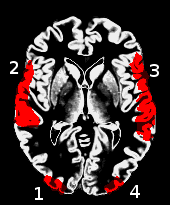
\includegraphics[width=3cm]{images/simregions.png}\label{fig:simslice_mask}}
\hfil
\subfloat[Mutual Information Map. Scale is bits. Higher (yellow) is better.]
{\label{fig:sim_hm_mi} 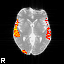
\includegraphics[width=4cm]{images/sim_hm_15_6.png}}
\subfigure{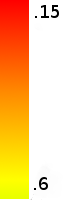
\includegraphics[width=.6cm]{images/scale6.png}}
\caption{Comparison of activation with greymatter, parameter regions.}
\label{fig:simslice_hm}
\end{figure}

%todo fix these histograms with marker for true value and drop A1,A2
\begin{figure*}[!t] %top left
\centering
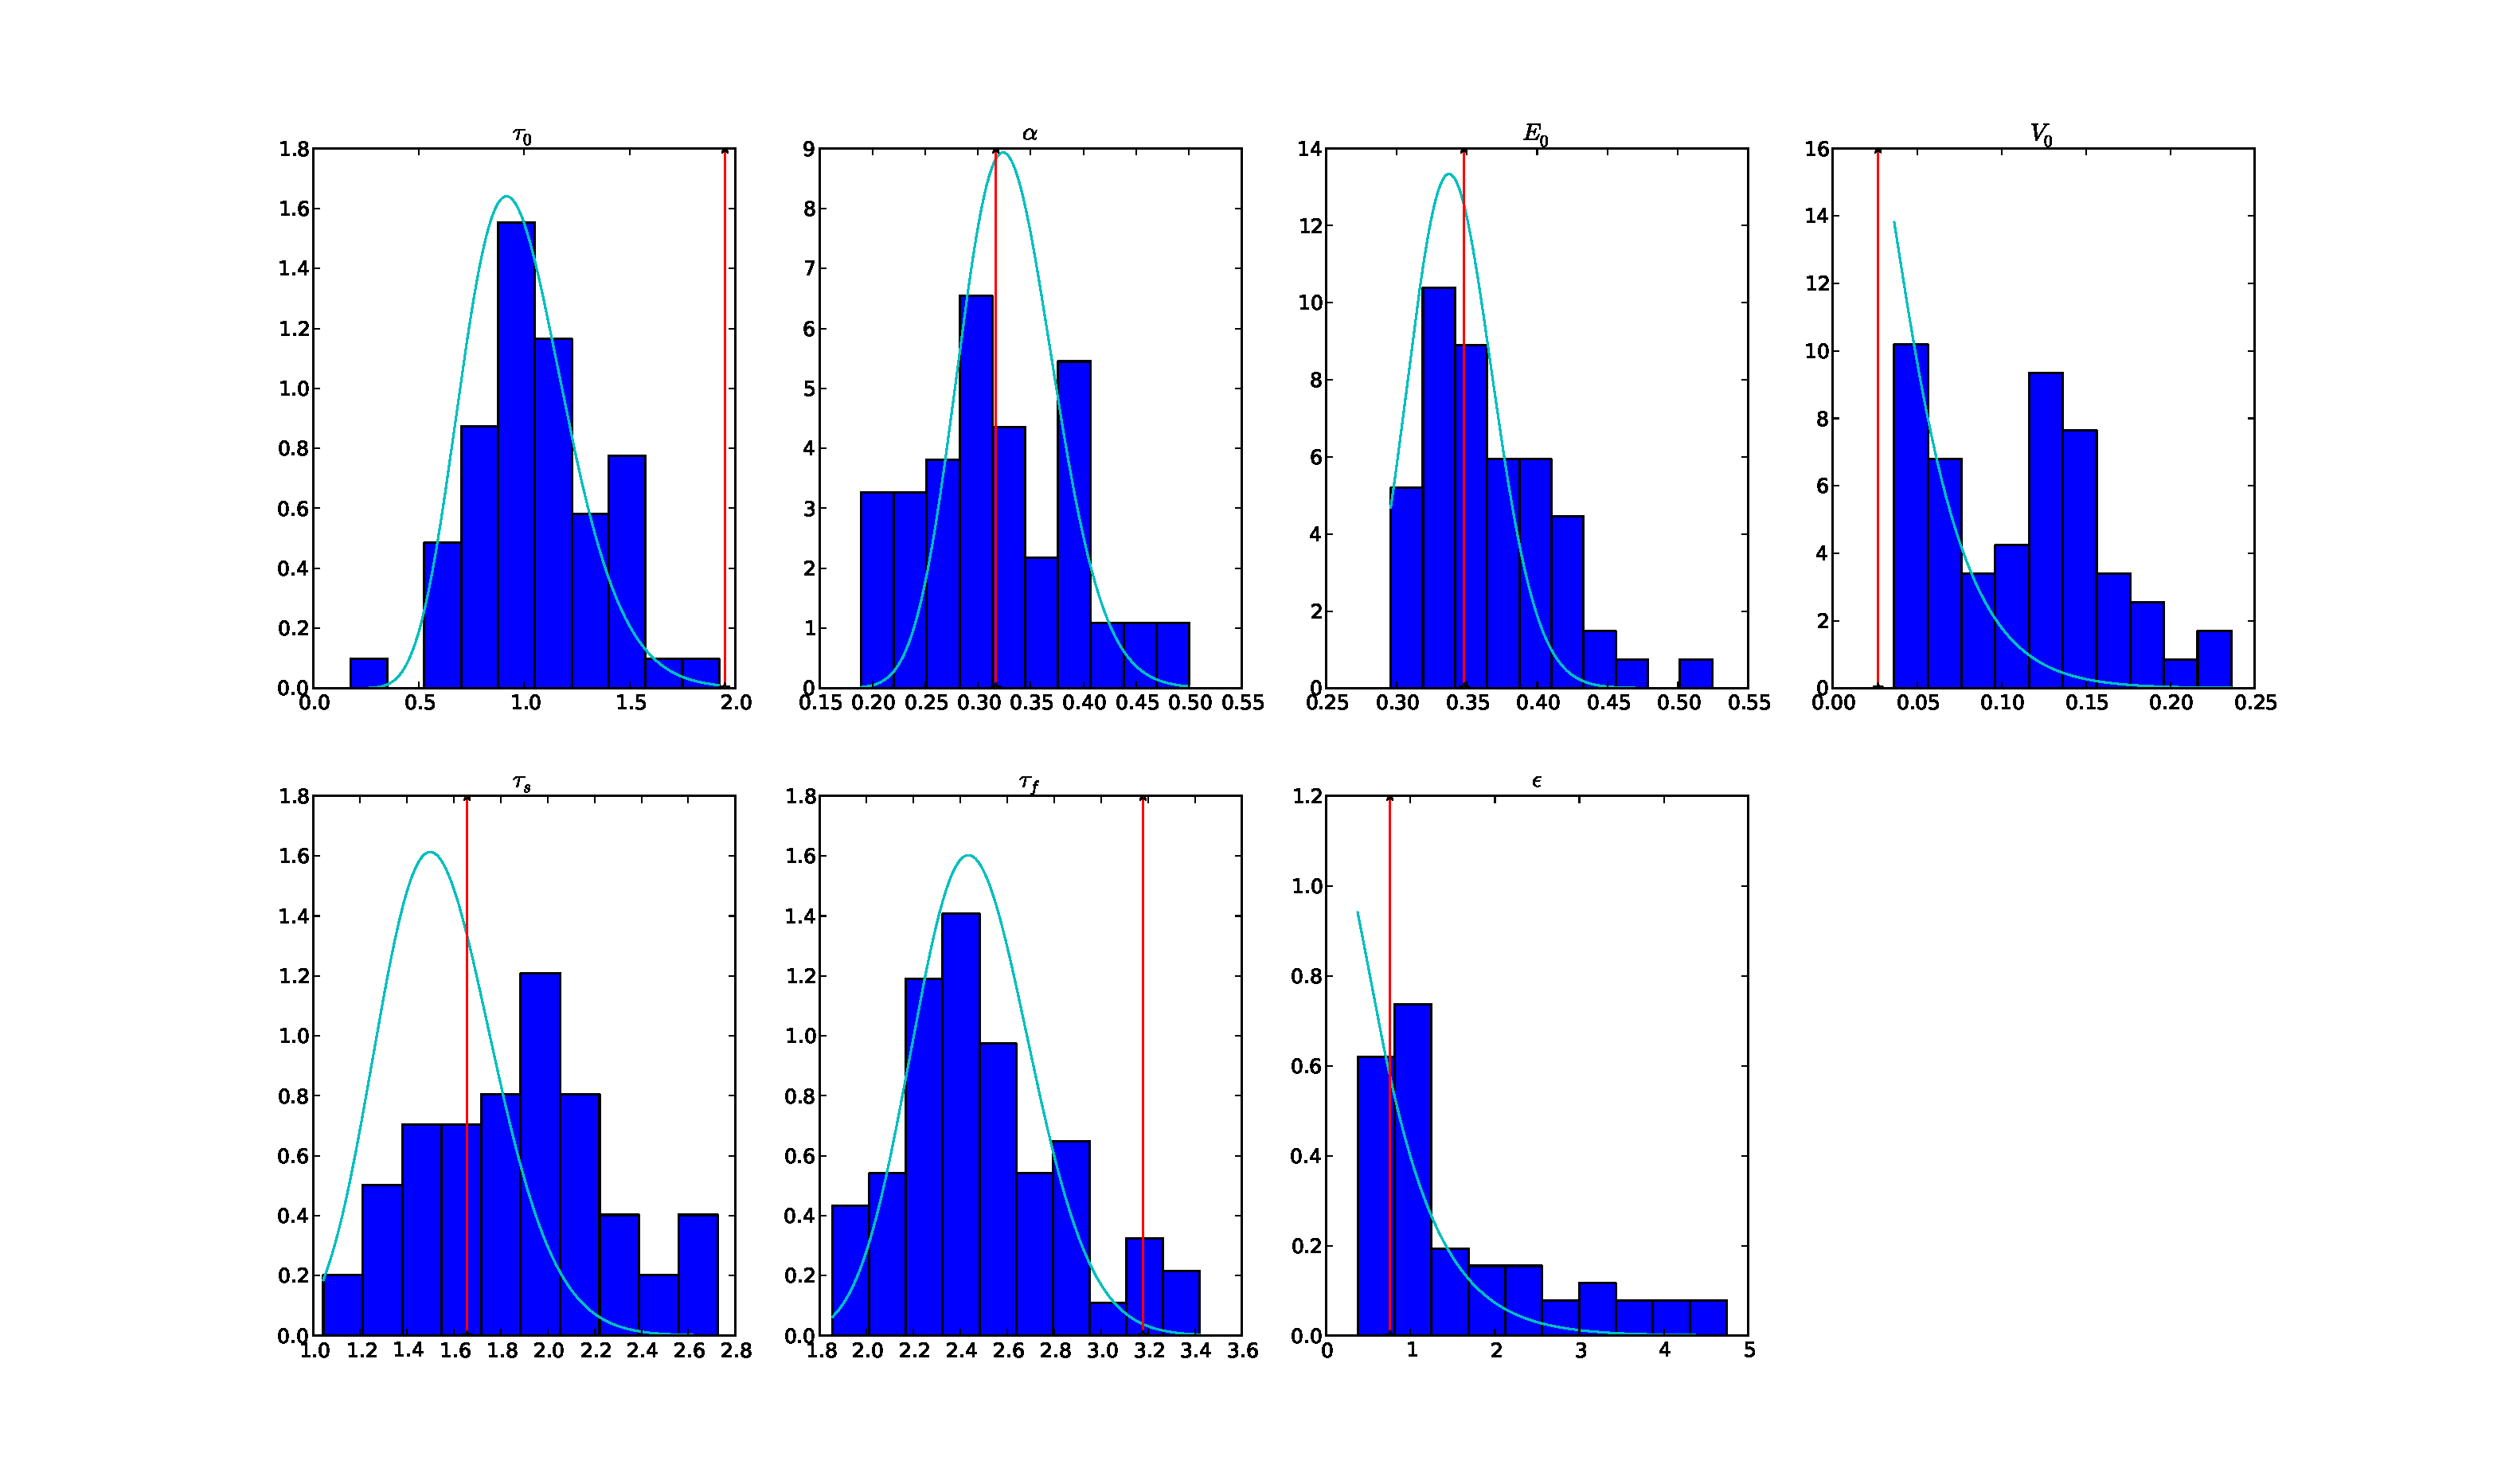
\includegraphics[clip=true,trim=2.5cm 2cm 2cm 1cm,width=15cm]{sec2hist}
\caption{Histogram of estimated parameters. Average SNR in the region was 
$0.97$ and Mutual Information between simulation and BOLD estimate was greater 
than $0.15$.}
\label{fig:slicesim_hist2}
\end{figure*}

\begin{figure*}[!t] %top left
\centering
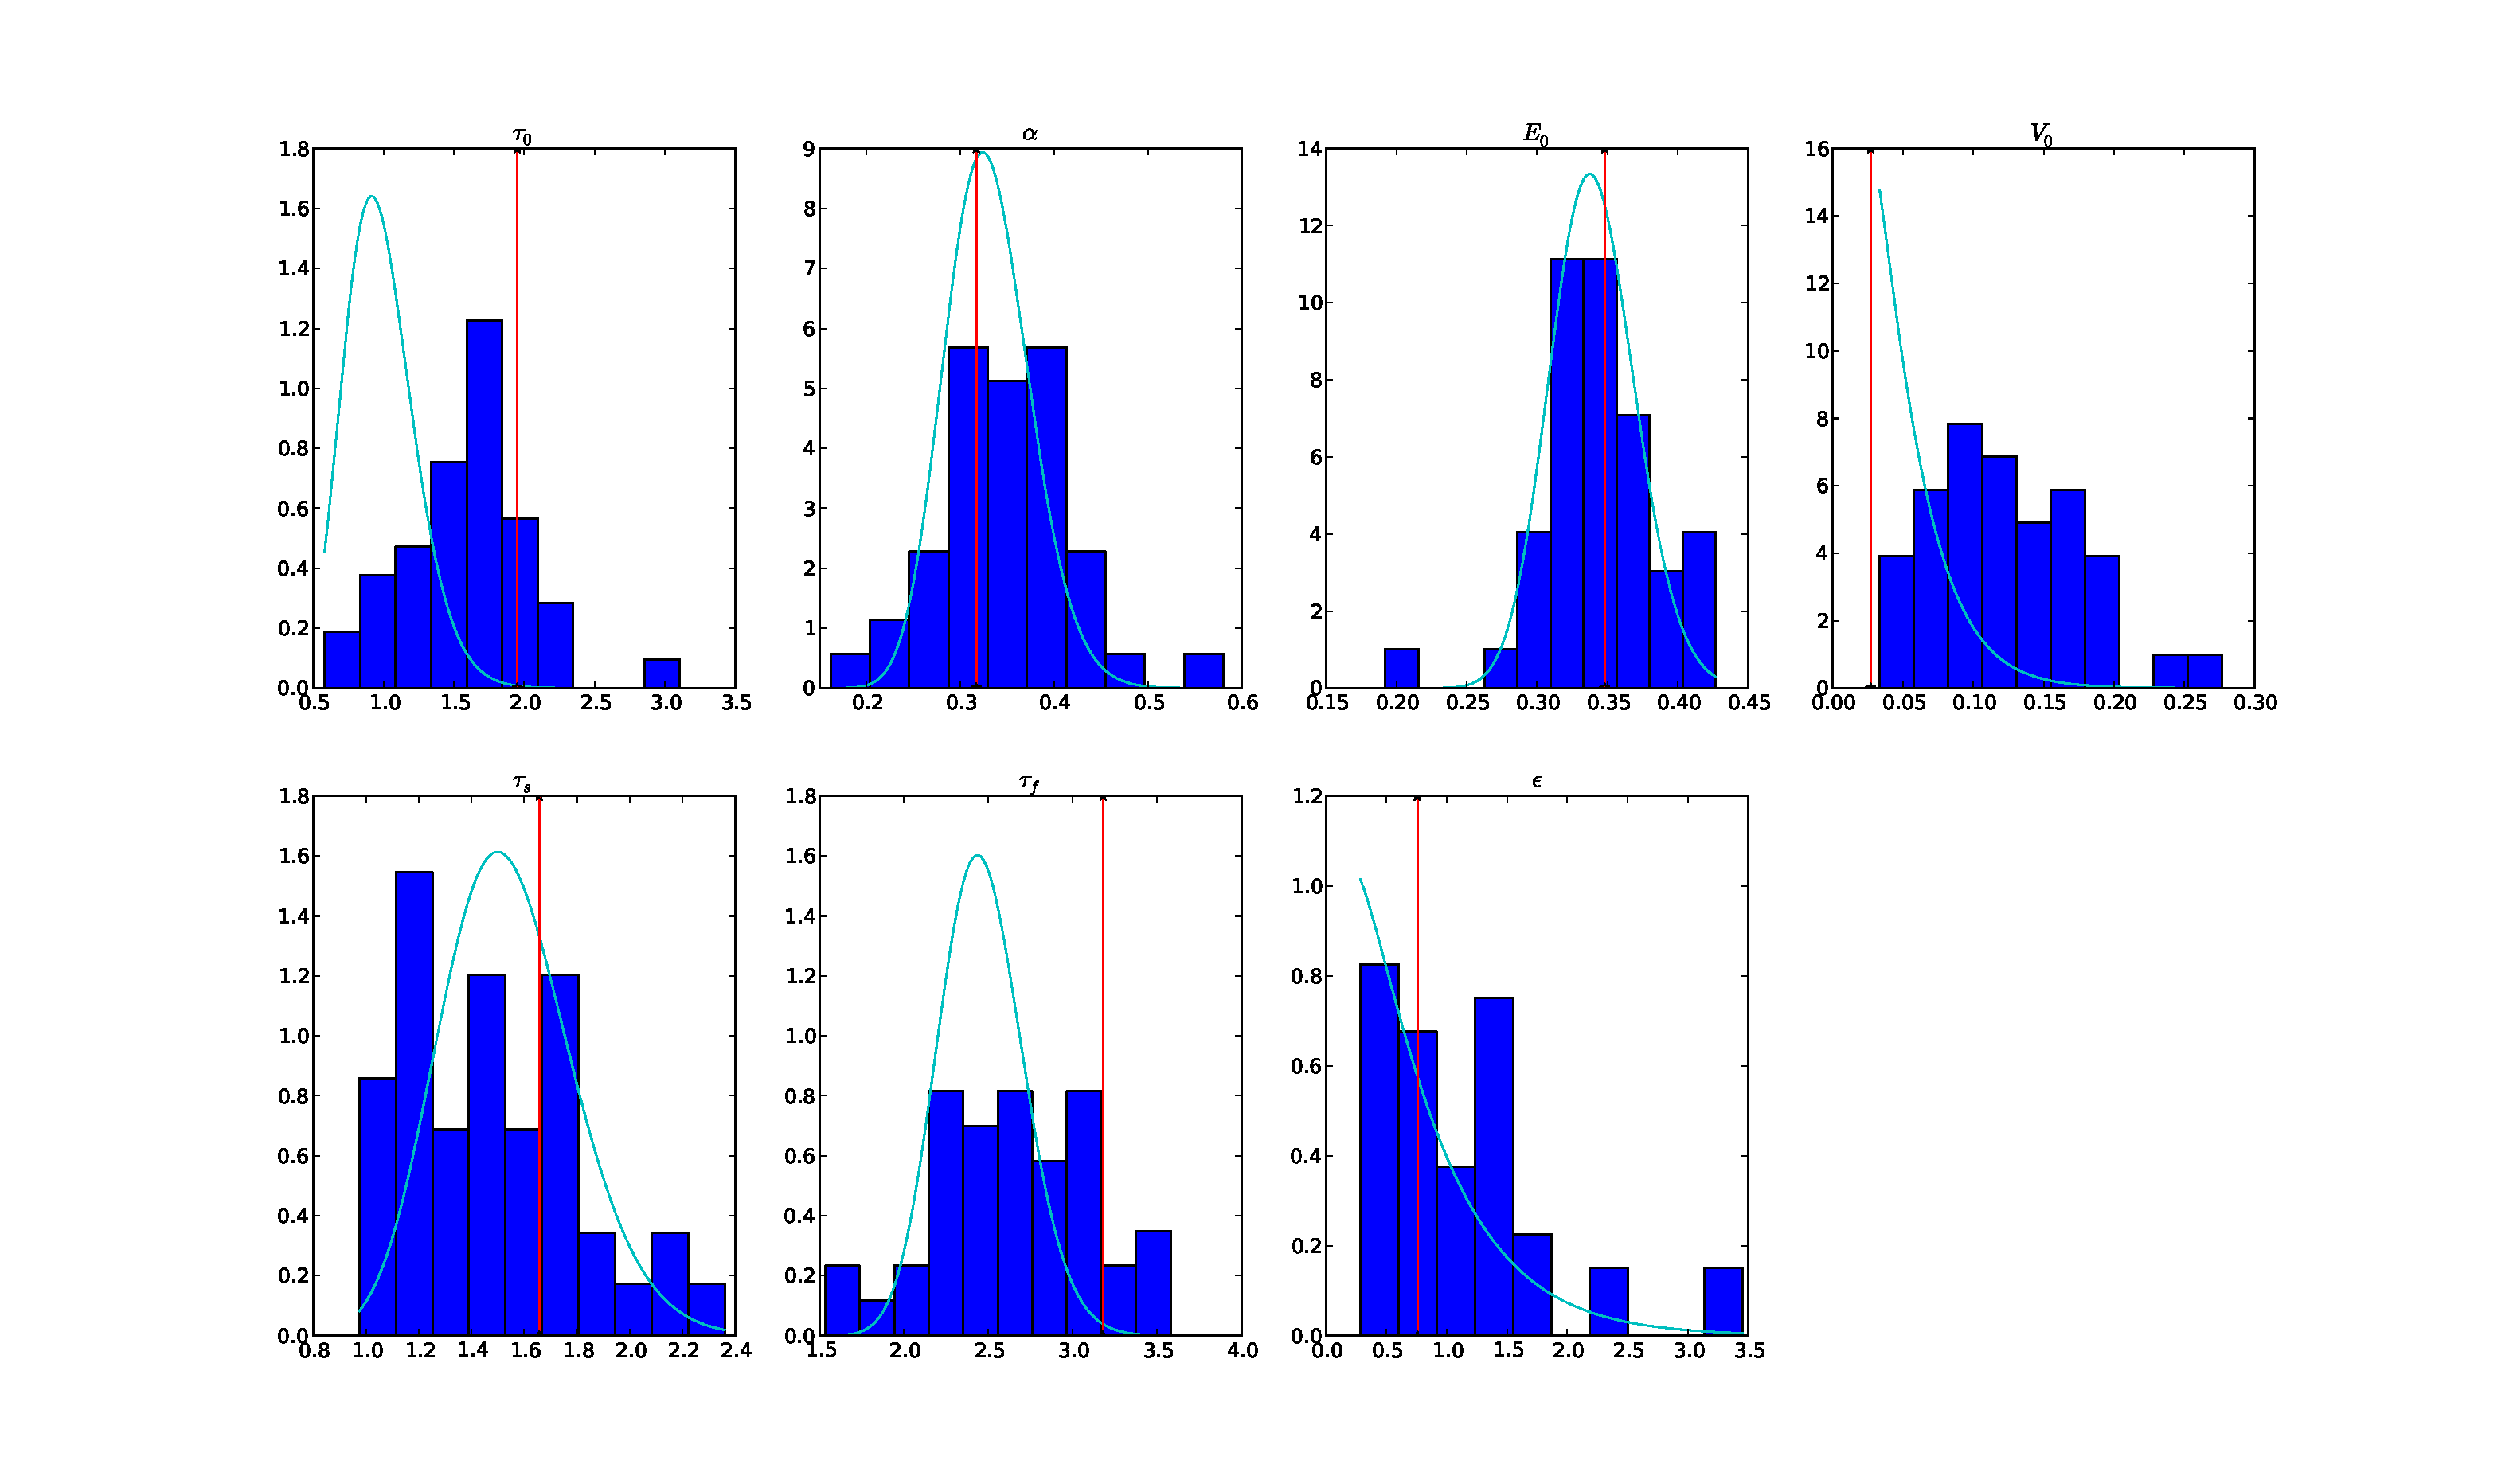
\includegraphics[clip=true,trim=2.5cm 2cm 2cm 1cm,width=15cm]{sec3hist}
\caption{Histogram of estimated parameters for region 3. Average SNR in the 
region was 
$0.39$ and Mutual Information between simulation and BOLD estimate was greater 
than $0.15$.}
\label{fig:slicesim_hist3}
\end{figure*}

In the POSSUM simulation, areas passing a threshold of
mutual information of $0.15$  are shown in 
\autoref{fig:sim_hm_mi}
whereas the active region numbers are shown in 
\autoref{fig:simslice_mask}.
Note that region 4 had a very small $\epsilon$ and so
had an extremely low $SNR$ ($<.1$). The histograms of parameter
estimates for sections
2 and 3 are shown in \autoref{fig:slicesim_hist2} and 
\autoref{fig:slicesim_hist3}, respectively. Region 1 is
left out because of the low number of points and because
its SNR was between region 2 and region 3 ($0.8$), so it
was a less interesting result.

\subsection{Real Data}
\begin{figure*}
\centering
\subfigure{\label{fig:hm_spm} 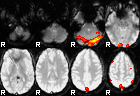
\includegraphics[scale=3]{spm_hm}}
\subfigure{\label{fig:scale_spm} 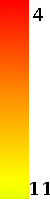
\includegraphics[scale=.35]{scale1}}
\caption{SPM results. Units of activation are in Student's $t$-scores; higher indicates higher
        assurance that the signal cannot have occurred through noise alone.}
\label{fig:hm_canon_spm}
\end{figure*}

\begin{figure*}
\centering
\subfigure{\label{fig:hm_mi} 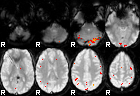
\includegraphics[scale=3]{hm_mi_strict}}
\subfigure{\label{fig:scale_mi} 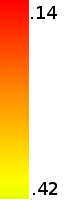
\includegraphics[scale=.35]{scale4}}
\caption{Particle filter results. Units of activation are in mutual information; higher
    indicates more assured activation.}
\label{fig:hm_canon_spm}
\end{figure*}

The result of real experiments concentrates on regions of activation, because
of the significant possiblity that the parameters are strictly defined. The
quality of fit used for the particle filter results is mutual information which
in preliminary testing showed fewer false positives than normalized Mean Squared
Error. 

\section{Discussion}
\label{sec:Discussion}

\section{Conclusion}
\label{sec:Conclusion}

%This article is organized as follows. The rest of the introduction will
%overview similar efforts and discuss their strengths ans weaknesses.
%\autoref{sec:Bold Model} will describe the genesis of the BOLD model,
%and its current state. \autoref{sec:Particle Filter} will explain the 
%particle filter and how it is being used in this case. 
%\auroref{sec:Methods} will describe in detail the experimental
%design, algorithm set up, and the preprocessing that was applied
%for the particle filter algorithm.
%The results are explored separately for simulated data
%and real FMRI data in \autoref{sec:SimulationResults} and 
%\autoref{sec:RealData}, respectively. 
%In \autoref{sec:Discussion} the results and their implications 
%for future works are interpreted. 

\appendices

\section{Particle Filter Algorithm}
\label{sec:algorithms}

\subsection{Sequential Importance Sampling}
\label{alg:BasicParticleFilter}
\begin{algorithm}
\begin{algorithmic}
\STATE Initialize Particles:
\FOR{$i$ : each of $N_p$ particles }
    \STATE $x^i_0  \sim \alpha(X)$
    \STATE $w^i_0 = \frac{1}{N_p}$
\ENDFOR
\FOR{$k$ : each measurement}
    \FOR{$i$ : each particle }
        \STATE $x^i_k = x^i_{k-1} + \int_{t-1}^t f(x(\tau), u(\tau)) d\tau $
        \STATE $w^i_k = w^i_{k-1}P(y_k | x_k)$
    \ENDFOR
\ENDFOR
\begin{equation*}
\begin{array}{l}
P(x(t_k+\Delta t)) \approx \\
\sum_{i=0}^{N_p} w^i_k \delta\left(x - x^i_k - \int_{t_k}^{t_k+\Delta t} f(x(\tau), u(\tau)) d\tau \right) 
\end{array}
\end{equation*}
\end{algorithmic}
\end{algorithm}

\subsection{Resampling Algorithm}
\label{alg:RegResampling}
\begin{algorithm}
\begin{algorithmic}
\STATE Calculate total weight, $W_t = \sum_{i=0}^{N_p} w^i$
\FORALL{$0 < i < N_p$}
    \STATE Draw $V$ from uniform range $[0, W]$
    \STATE $C = W_t$
    \FORALL{$0 < j < N_p$ and $C < V$}
        \STATE $C = C - w^j$
    \ENDFOR
    \STATE Add $[x^j, \frac{1}{N_p}]$ to the new distribution
\ENDFOR
\STATE 
\end{algorithmic}
\label{alg:Resampling}
\end{algorithm}

\subsection{Regularized Resampling Algorithm}
\label{alg:RegResampler}
\begin{algorithm}
\begin{algorithmic}
\STATE Calculate Covariance, $C$, of empirical distribution, $\hat{x}$
\STATE Find $D$ such that $DD^T = C$
\STATE Resample $\hat{x}$ using algorithm from \autoref{alg:Resampling}
\FOR{$0 < i < N_p$}
    \STATE Draw $\epsilon$ from the standard normal, same dimensionality as $X$
    \STATE $x^i = x^i + hD\epsilon$
\ENDFOR
\end{algorithmic}
\end{algorithm}

\subsection{Regularized Particle Filter}
\label{alg:RegularizedParticleFilter}
\begin{algorithm}
\begin{algorithmic}
\STATE Initialize Particles:
\FOR{$i$ : each of $N_p$ particles }
    \STATE $x^i_0  \sim \alpha(X)$
    \STATE $w^i_0 = \frac{1}{N_p}$
\ENDFOR
\FOR{$k$ : each measurement}
    \FOR{$i$ : each particle }
        \STATE $x^i_k = x^i_{k-1} + \int_{t-1}^t f(x(\tau), u(\tau)) d\tau $
        \STATE $w^i_k = w^i_{k-1}P(y_k | x_k)$
    \ENDFOR

    \STATE Calculate $N_{eff}$ with \autoref{eq:neff}
    \IF{$N_{eff} < N_R$ (recommend $N_R = min(50, .1N_p)$ )}
        \STATE Resample using algorithm from \autoref{alg:RegResampling}
    \ENDIF
\ENDFOR

\STATE At $t + \Delta t$, $t \in T$, $P(x(t+\Delta t)) \approx 
\sum_{i=1}^{N_p} w_i(t)\delta\left(x - (x_i(t) + \int_t^{t+\Delta t} f(x(\tau), u(\tau)) d\tau) \right)$
 \end{algorithmic}
 \end{algorithm}

% you can choose not to have a title for an appendix
% if you want by leaving the argument blank
\section{}
Appendix two text goes here.


% use section* for acknowledgement
%\section*{Acknowledgment}

\bibliographystyle{IEEEtran}
\bibliography{IEEEabrv,./library}

\end{document}
